\chapter{Tests und Experimente}
In diesem Kapitel werden Experimente mit den drei Datensätze durchgeführt. Ebenfalls werden verschiedene Hyperparameter getestet.

\section{Spiel-Datensatz Experimente}
Als erstes wird die Methode auf dem Spiel-Datensatz angewendet. Hiermit soll geprüft werden ob die Methode die erwartete
Ergebnisse liefert. Das U-Net wird für 100 Epochen mit Adam, eine Lernrate von 0.001 und die Cross Entropy Loss Funktion trainiert. Dieser
Einstellung erwies die besten Ergebnisse. Außerdem wurde ein Experiment mit 36 und ein mit 324 Bins durchgeführt, was kein Einfluss auf die 
Ergebnisse vorwies. Es kann davon ausgegangen werden, dass bei der niedrige Anzahl an möglichen Farben, ein Unterschied bei 36 und 324 Bins
nicht zu erkennen ist. Die unteren Ergebnissen wurden mit 324 Bins erstellt.

\begin{figure}[H]
  \vspace{1cm}
  \begin{subfigure}
    \centering
    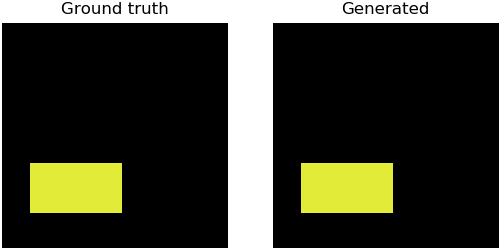
\includegraphics[width=.32\textwidth]{resources/experiments/30.png}
  \end{subfigure}
  \begin{subfigure}
    \centering
    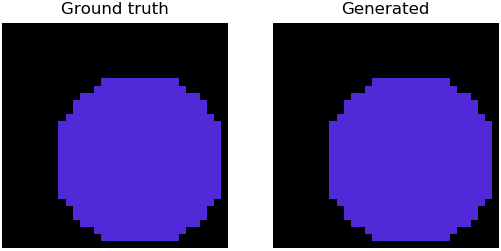
\includegraphics[width=.32\textwidth]{resources/experiments/31.png}
  \end{subfigure}
  \begin{subfigure}
    \centering
    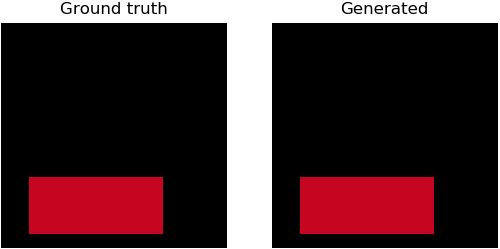
\includegraphics[width=.32\textwidth]{resources/experiments/42.png}
  \end{subfigure}
  \caption{Beispiele von sehr gute Ergebnisse aus dem Spiel-Datensatz}
  \label{image:gute-ergebnisse-toy-dataset}
\end{figure}

Bei den oberen Ergebnisse wurden alle Pixeln richtig klassifiziert, was bei der Größe des Datensatzes oft zu overfitting deutet.
Die unteren Ergebnissen zeigen dass das Model generalisiert und nicht overfitet hat.

\begin{figure}[H]
  \vspace{1cm}
  \begin{subfigure}
    \centering
    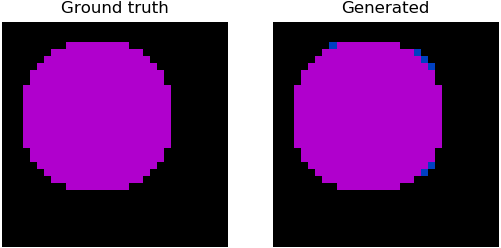
\includegraphics[width=.32\textwidth]{resources/experiments/581.png}
  \end{subfigure}
  \begin{subfigure}
    \centering
    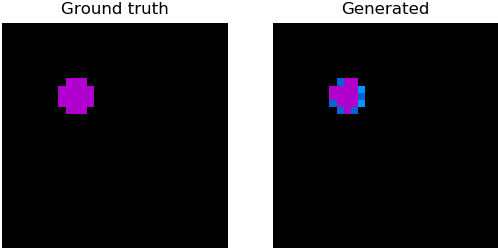
\includegraphics[width=.32\textwidth]{resources/experiments/712.png}
  \end{subfigure}
  \begin{subfigure}
    \centering
    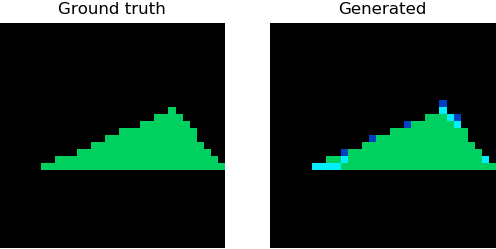
\includegraphics[width=.32\textwidth]{resources/experiments/761.png}
  \end{subfigure}
  \caption{Beispiele von generalisierte Ergebnisse}
  \label{image:nicht-gute-ergebnisse-toy-dataset}
\end{figure}

Das Model hat bei einige Ergebnisse, Schwierigkeiten die Pixeln am Rand der geometrische Formen, richtig zu klassifizieren.
Dies tritt speziell auf die Kreise und Dreiecke wo die Ränder nicht glatte Linien sind.
\\
Die Ergebnisse bestätigen dass das Binning und die Methode funktionieren. Anschließend wurden Experimente auf komplexere Bilder
von dem Subset von CIFAR-100 durchgeführt.

\section{CIFAR-100 Subset Experimente}
Das Model wurde auf 12 Klassen von CIFAR-100 über 100 Epochen mit Adam, eine Lernrate von 0.001 und die Cross Entropy Loss Funktion
trainiert.


% \begin{figure}[H]
%   \centering
%   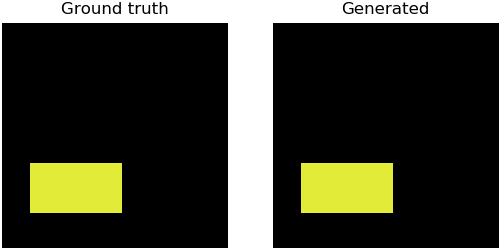
\includegraphics[width=1\textwidth]{resources/experiments/30.png}
%   \caption{
%   \gls{grid} mit 36 bins. Die x-Achse bildet die Werte von dem Farbkanal ``a'' und die y-Achse die Werte von den Farbkanal ``b'' ab.
%   }
%   \label{image:bins}
% \end{figure}